\section{Prosjektplan}

\subsection{Utviklingsmetode}

Prosjektgruppe har valgt Scrumban som utviklingsmetode. Scrumban er en hybrid av Scrum og Kanban som benytter Backlog for planlegging, prioritering og fordeling av arbeidsoppgaver og Kanban board for visualisering av prosjektets framgang \cite{6-scrumban-overview}.

%Figur - Scrumban prosessen.
\begin{figure}[ht]
\centering
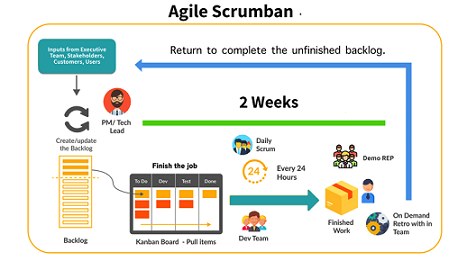
\includegraphics{images/fig-scrumban.png}
\caption{Scrumban prosessen \cite{6-scrumban-overview}}
\label{fig:fig-scrumban}
\end{figure}
 

Scrumban er iterativ prosess som kan deles inn i korte perioder. Lengde av hver periode kan variere fra en til fire uker og bestemmes av prosjektgruppen. Vanligvis tar en periode cirka 2 uker \cite{6-scrum-vs-kanban-vs-scrumban}.

Som en del av Scrumban prosess etableres det en Backlog. Den inneholder en liste over elementer som kan bli utviklet i løpet av prosjektperioden. Antall elementer i Backlogen varierer, og nye elementer kan bli lagt til når som helst \cite{6-scrum-vs-kanban-vs-scrumban}.

Elementene har prioritering og WIP begrensning. WIP står for «work-in-progress limit» og setter en grense for antall oppgaver som skal plasseres i «in progress» kolonne av Kanban board. Elementene med høyest prioritet skal utføres først \cite{6-scrum-vs-kanban-vs-scrumban}. Scrumban Board er presentert i figur \ref{fig:fig-scrumban-board}.

 
%Figur - Scrumban Board
\begin{figure}[ht]
\centering
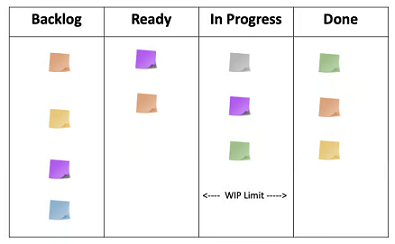
\includegraphics{images/fig-scrumban-board.png}
\caption{Scrumban Board. WIP begrensning i "in progress" kolonne. \cite{4-logrocket.com-scrumban}}
\label{fig:fig-scrumban-board}
\end{figure}
 

Kanban board brukes til visualisering av kontinuerlig arbeidsflyt. Elementene fra Backlogen plasseres og tas av gruppemedlemmer etter pull prinsippet. Etter at man er ferdig med sin oppgave, tar en ny fra tavlen \cite{6-scrum-vs-kanban-vs-scrumban}.

Prosjektgruppen skal møtes hver dag for korte stand-up møter. Målet med disse møtene er å gå gjennom gjennomført og pågående arbeid, se gjennom en liste med prioriterte oppgaver og finne løsninger til eventuelle problemer \cite{4-logrocket.com-scrumban}.

På slutten av iterasjonen, samles prosjektgruppe for å diskutere gjennomført arbeid, implementert funksjonalitet, eventuelle mangler, tilleggskrav fra kunden, utviklingsprosess og nødvendig forbedringstiltak som vil gjøre prosjektgruppe mer produktiv neste iterasjon \cite{6-agilealliance-scrumban}.

Etter det starter prosjektgruppe planlegging av en ny iterasjon, justering og prioritering av elementer i Backloggen \cite{6-agilealliance-scrumban}.

\subsection{Jira Software}

Jira Software er et prosjektstyring verktøy som skal brukes til å støtte Scrumban prosessen. Prosjektet lages ved hjelp av Kanban Project Template. Ved å velge Team-Managed Template, kan man gjøre styring av prosjektet mer fleksibelt. Det finnes også mulighet til å koble GitHub repository til prosjektet \cite{4-atlassian.com-jira}.

Kanban board bukes til styring av prosjektarbeid. Den er delt inn i tre kolonner: TO DO, IN PROGRESS og DONE. Det er mulig å endre navn eller legge til ekstra kolonner, for eksempel BACKLOG \cite{4-atlassian.com-jira}.

Elementene fra Backloggen plasseres på tavla. Kanban prosjekt har tre hovedtyper elementer: epics, tasks og subtasks. Epics brukes til gruppering av elementer og kan bli koblet sammen ved hjelp av avhengigheter. Tasks er en primær type element og kan bli delt inn i mindre subtasks \cite{4-atlassian.com-jira}.

Prosjektgruppe styrer sitt arbeid ved å ta og flytte arbeidsoppgaver på forskjellige steder av Kanban board. Oppgavene skal utføres etter høyest prioritet. Kanban board er presentert i figur \ref{figur:kanban-board}.

%Figur - Kanban Board
\begin{figure}[ht]
\centering
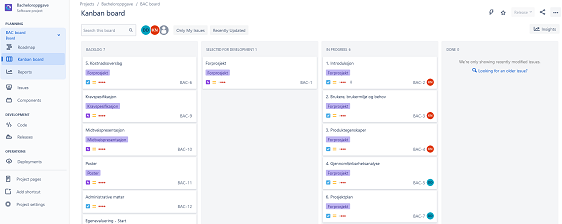
\includegraphics{images/kanban-board3.png}
\caption{Kanban Board. Generert med Jira Software.}
\label{figur:kanban-board}
\end{figure} 

\newpage
Kanban roadmap som er presentert i figur \ref{figur:kanban-roadmap} gir en oversikt over alle Epics og viser hvor lang tid en bestemt Epic tar i løpet av utviklingsprosessen \cite{4-atlassian.com-jira}.   

%Figur - Kanban Board
\begin{figure}[ht]
\centering
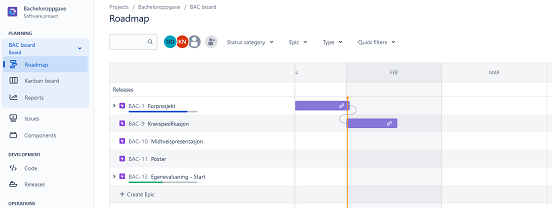
\includegraphics{images/kanban-roadmap3.png}
\caption{Kanban Roadmap. Generert med Jira Software.}
\label{figur:kanban-roadmap}
\end{figure} 

Jira Software gir også mulighet til å lage diverse rapporter og grafer (Average Cycle Time), som blir til en stor hjelp ved ferdigstillelse av nødvendig dokumentasjon \cite{4-atlassian.com-jira}.

